
% Currently supported format is the old 4:3 aspect ratio (and not for 16:9)
% You need to select the LuaTeX engine to compile to pdf, perhaps XeTeX would also work
% If you use Overleaf, you have to change the compiler (https://www.overleaf.com/learn/how-to/Changing_compiler)
% Reason: The common pdfTeX engine cannot use system fonts: Calibri, Georgia

\documentclass[aspectratio=43]{beamer}

% Load package "amsmath" before PSI43 (because "fontspec" inside PSI43 should be loaded before "amsmath" according to an advice)
\usepackage{amsmath}

\usepackage[blockcolored]{PSI43} % blockcolored is required if you want to ahve colored blocks, because the default beamter theme has uncolered boxes







\begin{document}

\title{A novel approach to energy system analysis and technology assessment}

\author[L. Wittgenstein]{Ludwig Wittgenstein}
% if short author is given in options, it will be taken for the footline

\institute[LEA, PSI]{Laboratory of Energy Systems Analysis, Paul Scherrer Institute}
% if short institute is given in options, it will be taken for the footline

\subtitle{1st Line\\2nd Line (a 3rd line may be required for single-line titles to move gray box down)}

\date{LEA Seminar, 1.1.2021} % can be left empty

\begin{frame}[plain] % plain prohibits logo, footer etc.
  \titlepage
\end{frame}


\begin{frame}{A list that is reveiled}  
  \begin{itemize}
  \item<1-> Item 1
  \item[-]<1->  Item 1 (with dash instead of bullet)
    \begin{itemize}
    \item<1-> Item 1b
    \end{itemize}
  \item<2->  Item 2 (revealed on next slide)
  \item<3-> Item 3
    \begin{itemize}
    \item<3-> Item 4
      \begin{itemize}
      \item<3-> Item 5
      \end{itemize}
    \end{itemize}
  \end{itemize}
 \vspace*{\fill} % to put the text a little bit upwards
\end{frame}



\begin{frame}[squeeze]{Titles over two lines are possible (just the PSI logo is a little bit down)}
  \alert{This is a frame with the usual `squeeze' option of beamer to narrow linespacing a little bit, The color of this text is called ``alert'' in beamer}
  
  \structure{This is a color predefined in beamer called ``structure''}
  \begin{align*}
    a + b  & = \int_a^b f(x)\,dx \\
    \sum_{n=1}^N x_{i_n} &= \frac{a+b}{c+d} 
  \end{align*}
  \begin{itemize}
  \item  $\alpha = \zeta$ 
  \item $\mathcal{F}_t$, $\mathbb{R}^n$
  \item $\{t \mid t=1,\dots,T\}$
  \item $f\colon x\to y$
  \end{itemize}  
\end{frame}

\begin{frame}{Columns and Blocks}
  You can start text very high with the space command with the code in the  .tex file of this slide

  The color of the blocks are defined in the preamble of the .tex file:
  \begin{columns}
    \begin{column}[T]{4cm}
      \centering
      \begin{block}{Text in a block}
        This is a block of text in the first column
      \end{block}
      \begin{exampleblock}{Text in an example block}
        This is a block of text in the first column
      \end{exampleblock}
      Text outside of block in first column
    \end{column}
    \begin{column}[T]{4cm}
      \begin{block}{Text in a block}
        This is a block 
      \end{block}
      \begin{alertblock}{Text in an alert block}
        This is a block
      \end{alertblock}
      \begin{block}{}
        This is a block without title (not nice...)
      \end{block}
    \end{column}
  \end{columns}
    
    \PSIfill
 \end{frame}


 \begin{frame}{Text}
   \PSIvspace
  You can start text a little bit lower with the command in this slide
  \begin{figure}
    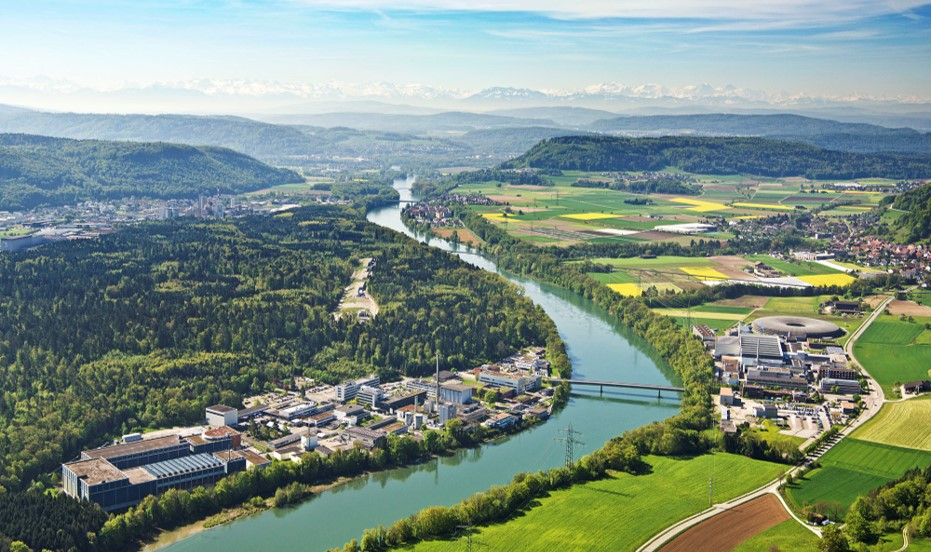
\includegraphics[width=0.3\pagewidth]{PSIlandscape}
    \caption{Figures are automatically centered}
    \label{fig:PSI}
    \end{figure}

     \PSIfill
\end{frame}

\PSItrailer{
    \textbf{My thanks go to}
     \smallskip
    \begin{itemize}
    \item Co-author 1
    \item Co-author 2 who has a very long name 
    \item Supervisor 1
    \item Supervisor 2  
    \end{itemize}
    }
  

\end{document}

% The following can be deleted if not the EMACS editor is used for editing

%%%Local Variables:
%%% mode: latex
%%% TeX-master: t
%%% TeX-engine: luatex
%%% End:
